\documentclass[a4paper,english,12pt,bibliography=totoc]{scrreprt}

\usepackage[T1]{fontenc} %immer
\usepackage[utf8]{inputenc} %am
\usepackage{babel} %Anfang

\usepackage{enumitem} %Aufzählungen verändern

%Gleichungen verwenden
\usepackage{newtxtext}
\usepackage{amsmath}
\usepackage{amssymb}
\usepackage{mathptmx}
%\usepackage{txfonts}

\usepackage{listings}% code blocks
\usepackage[most]{tcolorbox}

%Querverweise
\usepackage{varioref} %immer
\usepackage{hyperref} %in dieser
\usepackage{cleveref} %Reihenfolge

\usepackage{booktabs} %schönere Tabellen
\usepackage{siunitx} %SI-Einheiten
\usepackage{tabularx} %Tabellen mit flexiblen Spalten	

\usepackage{graphicx} %Grafiken verwenden

\usepackage{lipsum} %Blindtext
\usepackage{subcaption}
\usepackage{afterpage}
\usepackage[headsepline]{scrlayer-scrpage} %Paket für Kopfzeilen
\usepackage{afterpage}
\usepackage{float}
\automark[subsection]{section}

\pagestyle{scrheadings}
\ihead{} % oben links
\chead{\leftmark} % oben Mitte
\ohead{} % oben rechts
\cfoot{\pagemark} % unten Mitte
\automark[section]{section} % Modified line

% Zu volle hboxen korrigieren
\tolerance 1414
\hbadness 1414
\emergencystretch 1.5em
\hfuzz 0.3pt
\widowpenalty=10000
\vfuzz \hfuzz
\raggedbottom

%Informationen über das Dokument
\date{\today}


\begin{document}


\begin{titlepage}
	\centering
	
\includegraphics[width=0.8\textwidth]{logo_uulm.png}
	
	\vspace{1cm}
	\LARGE 
	\Huge \textbf{Biophysics Laboratory Course}
	
	\vspace{1cm}
	\Large Experiment:

	\Huge \textbf{Protein labelling}
	
	\vspace{15mm}
	\Large Performed on 11.12.2023
	
	\vspace{5mm}
	\LARGE Group 8
	
	\vspace{1cm}
	\Large
	\begin{tabular}{rcl}
	\textbf{Haiyang Zhang} & and & \textbf{Nicolae Turcan}\\
	\href{mailto:student.1@uni-ulm.de}{haiyang.zhang@uni-ulm.de} & & \href{mailto:student.2@uni-ulm.de}{nicolae.turcan@uni-ulm.de}
	\end{tabular}
	
	\vspace{7mm}
	Supervisor: David Sinn
	
	\vfill
	\begin{tabular}{p{50mm}@{\hspace{5cm}}p{50mm}}
	\centering \underline{} & \centering \underline{} 
	%\hrulefill & \hrulefill 
	\end{tabular}
	
	\vspace{5mm}
	\normalsize \raggedright
	We hereby confirm that we have elaborated the present work independently and have detailed knowledge of the entire contents.
\end{titlepage}

\tableofcontents


\chapter{Abstract}
\label{cha:abstract}
Fluorescence-based techniques are vital in various scientific domains due to their sensitivity and specificity. Our experiment focused on labeling proteins with Alexa Fluor 546 using amino modification and subsequent gel filtration chromatography. Despite challenges, such as an unexpected volume discrepancy during gel filtration, we successfully calculated the labeling efficiency and other key quantitative parameters. Photosensitivity considerations were emphasized, highlighting the need to shield fluorophores like Alexa Fluor from excessive excitation cycles. Our findings underscore the importance of optimizing reaction conditions and addressing procedural issues for accurate fluorescence-based analyses. The next phase involves Fluorescence Correlation Spectroscopy (FCS) for conjugation validation, promising further insights into refining experimental protocols.
\chapter{Introduction}
\label{cha:intro}
Fluorescence is a phenomenon in which a molecule absorbs light energy at a specific wavelength and then re-emits the absorbed energy as light at a longer wavelength. This process occurs when electrons within the fluorophore, a molecule capable of fluorescing, absorb energy and transition to an excited state. As the electrons return to their ground state, they release the excess energy in the form of fluorescent light. The emitted light typically has a longer wavelength and lower energy than the absorbed light because of vibrational relaxation or dissipation and solvent reorganization around the molecule, this process is defined as a Stokes shift [8]. Fluorescence is widely utilized in various scientific and technological applications, including bioimaging, molecular labeling, and analytical techniques, due to its sensitivity and specificity ( sensitivity results from the choice of the fluorescing molecule, which in dependence on the use-case scenario, can have a high Quantum yield to achieve better Signal to Noise Ratio or Resistance to Bleaching for prolonged imaging or even a change in environment sensing trough average lifetime measurements of the emitted photons.
Specificity on the other hand can be achieved through careful molecular design to exploit Molecular Interactions as is the case for DAPI and Ethidium Bromide which act as DNA intercalants because of their size and chemical groups, or by associating dyes to Antibodies that are already specific to a certain epitope) 
Fluorescence-based techniques collectively contribute to the comprehensive exploration of biological systems, offering precise tools for the analysis of genetic material, molecular imaging of cell structures and function, and finally the study of dynamic cellular processes through Live Fluorescent Microscopy, for example:
\newline

FISH (Fluorescence In Situ Hybridization) [9] utilizes fluorescent probes to bind to specific DNA sequences, offering a powerful tool for genetic research, chromosomal analysis, and the detection of genetic abnormalities. This technique enables precise mapping of DNA within cellular structures.
\newline

FLIM (Fluorescence Lifetime Imaging Microscopy) [10] provides valuable insights into molecular environments by measuring the time a fluorophore spends in an excited state before returning to its ground state. This information distinguishes between single fluorophores and is instrumental in studying dynamic cellular processes at the molecular level.
\newline

FRET (Förster Resonance Energy Transfer) [11] relies on the transfer of energy between closely positioned fluorophores, allowing observation of molecular interactions by measuring the distance between labeled sites of a  macromolecule. Widely used for studying protein-protein interactions and conformational changes, FRET contributes to a deeper understanding of cellular dynamics.
\newline

Photosensitivity in fluorescence refers to the tendency of fluorophores, like those in "Alexa-Fluor Dyes" to undergo photobleaching after several excitation cycles. To mitigate this, proteins labeled with fluorophores should be protected from light, Here done by wrapping the container in aluminum foil instead of using Black-Plastic Eppendorfs. This precaution helps maintain fluorescence integrity during experiments.
\newline
\begin{figure}[H]
    \centering
    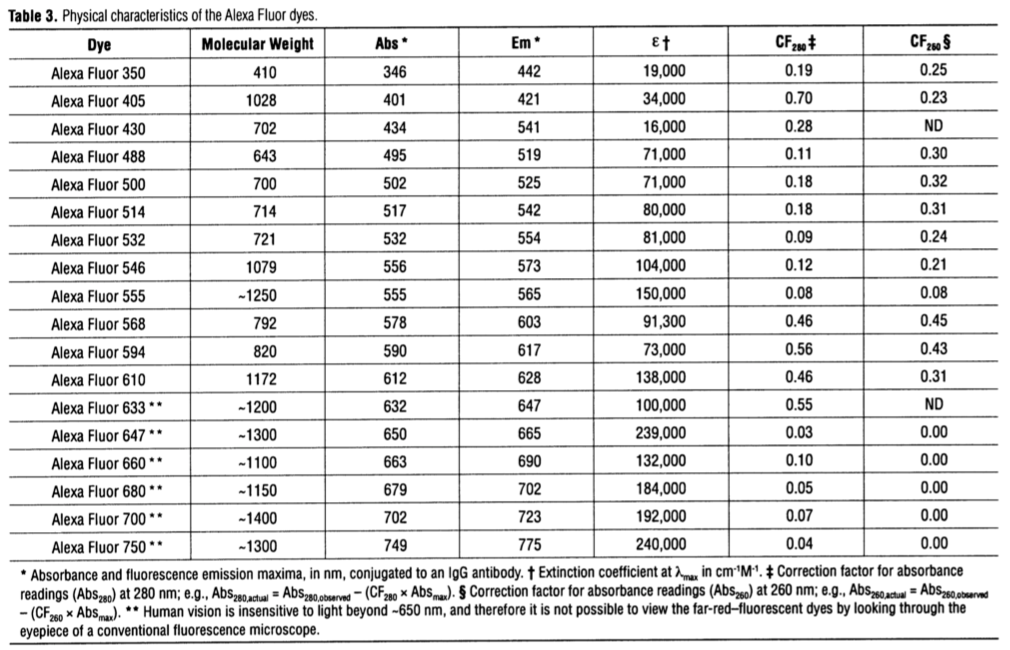
\includegraphics[width=0.8\textwidth]{alexafluordyes.png}
    \caption{AlexaFluor Fluorescent Dyes}
    \label{fig:ViolinPlot}
\end{figure}
Alexa Fluor 546 is a widely employed fluorescent dye recognized for its photostability and reliable signal strength and frequently utilized for biomolecule labeling in research applications, and thus empoloyed in the here presented experiment.

\begin{figure}[H]
    \centering
    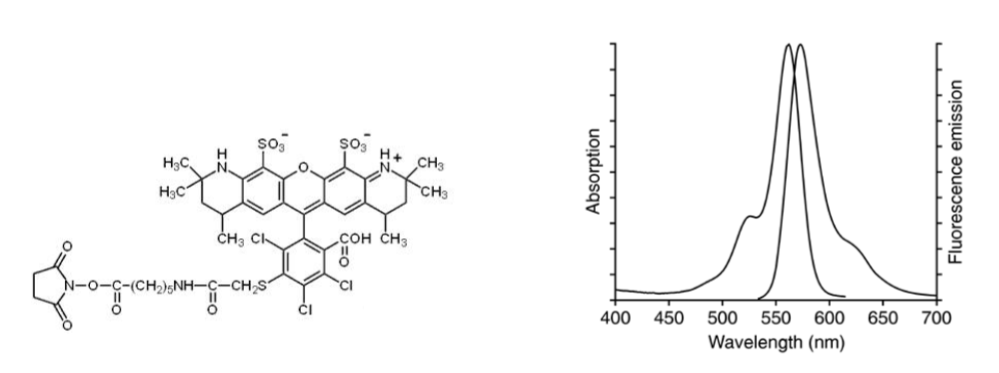
\includegraphics[width=0.8\textwidth]{alexafluor546.png}
    \caption{AlexaFluor546 NHS ester and absorption and emission spectrum}
    \label{fig:ViolinPlot}
\end{figure}


In our experiment, we utilized amino modification in conventional fluorescence for labeling proteins. This method provided stable conjugates due to the abundance of lysine in proteins, even though it wasn't suitable for site-specific labeling. The amino-reactive reagent is a product of the fluorophore Alexafluor 546  conjugated with succinimidyl ester (NHS ester) [12] was employed in this process. It is crucial to work in a slightly basic environment to ensure the deprotonation of amino groups, particularly the lysine Epsylon-amino groups with a pKa of about 10.5. Using a more neutral buffer might have resulted in the preferential reaction of succinimidyl ester with the Alpha-amino group, given its lower pKa compared to the Epsylon-amino group, resulting in binding of the yye at the N-terminus of the protein insted of the lysin side-chains.
\newline

The principle of gel filtration chromatography[1], where molecules are separated based on size using porous beads, bears a resemblance to molecular sieves. In both cases, smaller molecules can enter the pores and are retained longer, while larger molecules pass through more quickly.
In our experiment, we separated conjugates using gel filtration chromatography. The solid phase of the column consisted of swollen, small porous beads. Small molecules, including buffer molecules or the fluorescent dye, could penetrate into the bead pores and were retained longer than larger molecules, such as the proteins. The larger molecules flowed more quickly between the beads, causing them to elute early.

In the "spin columns" we utilized, centrifugal force increased the flow through the chromatography column. This accelerated flow facilitated the efficient separation based on size, allowing us to isolate and purify labeled proteins from unbound fluorescent dye or other smaller components.

\begin{figure}[H]
    \centering
    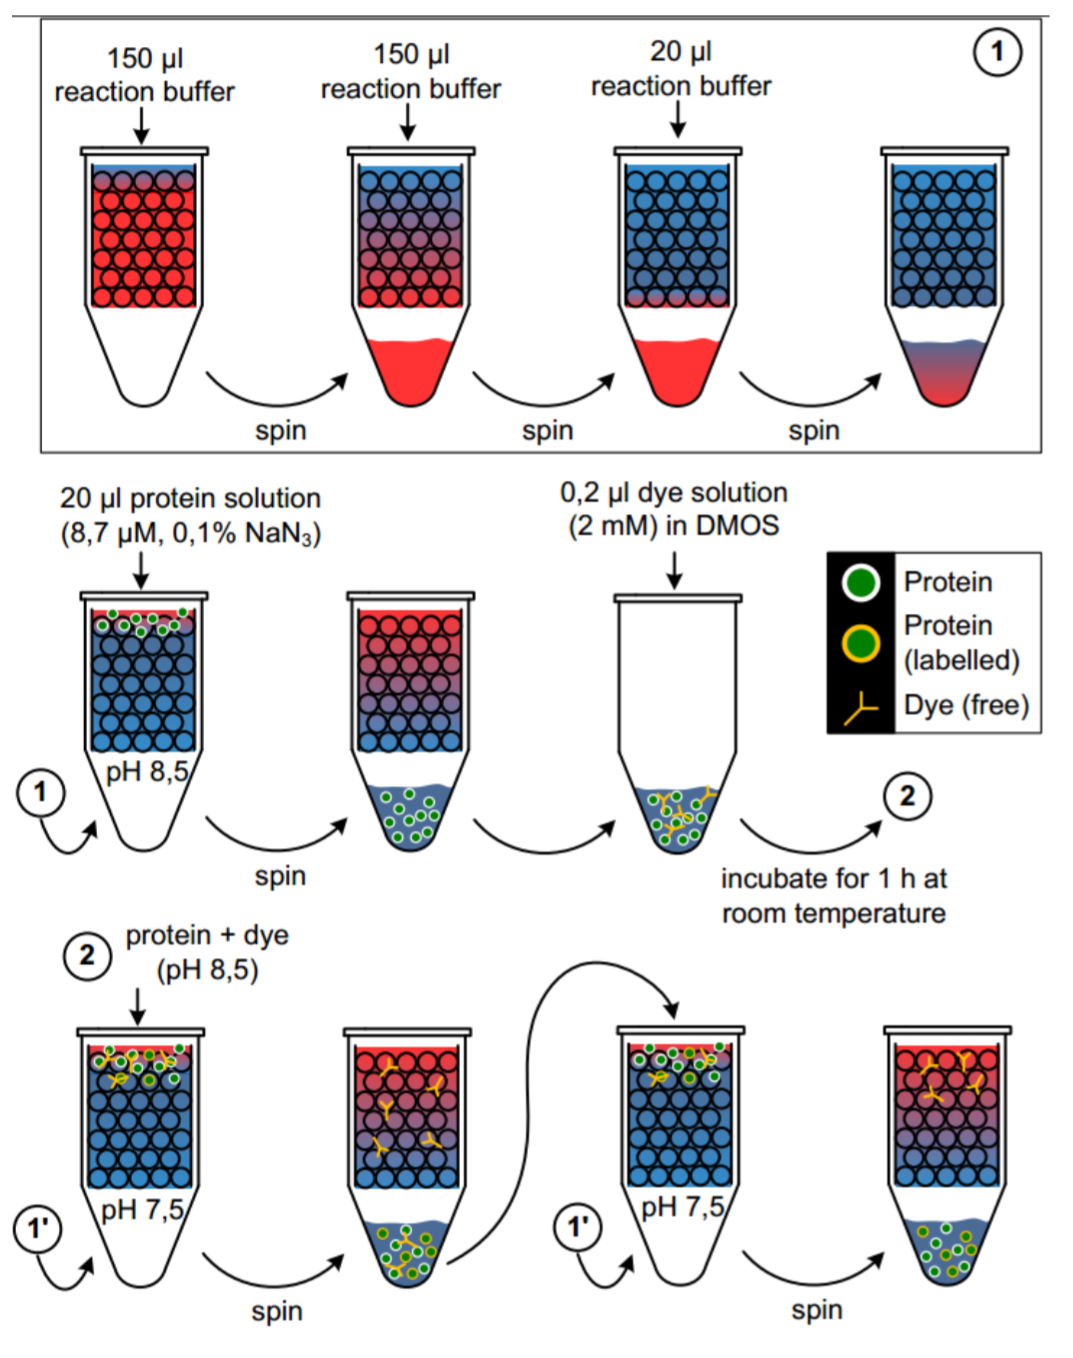
\includegraphics[width=0.75\textwidth]{spincolumnscheme.png}
    \caption{Spin Column Protocol}
    \label{fig:ViolinPlot}
\end{figure}


Derived from bovine blood, Bovine Serum Albumin (BSA) [13] is a widely used and well-characterized protein. Its stable structure and abundance of lysine residues make it a convenient target for labeling experiments. In our study, BSA served as the substrate for amino modification.

\begin{figure}[H]
    \centering
    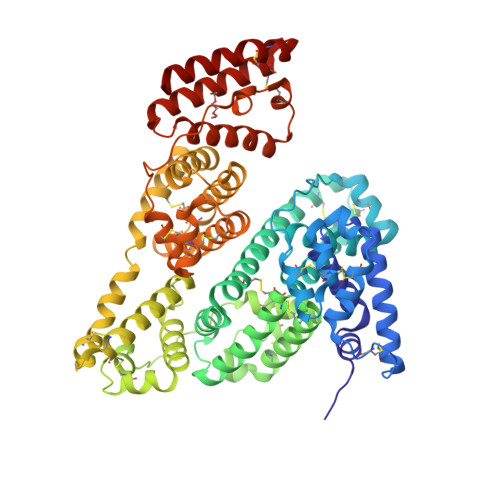
\includegraphics[width=0.8\textwidth]{Bovine Serum Albumin.jpeg}
    \caption{Bovine Serum Albumin Structure}
    \label{fig:ViolinPlot}
\end{figure}

\begin{figure}[H]
    \centering
    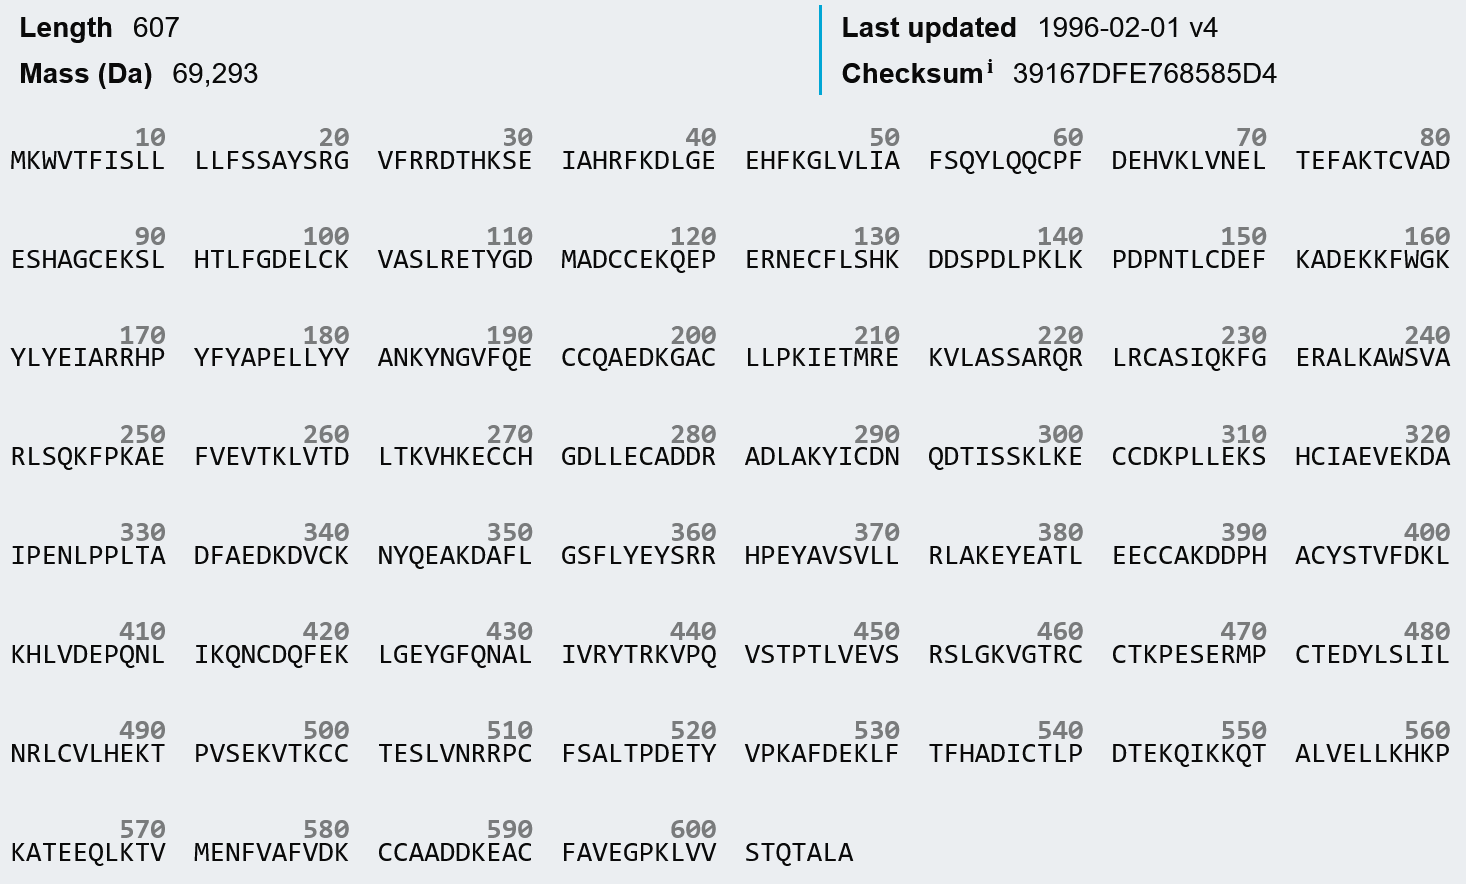
\includegraphics[width=0.5\textwidth]{sequence.png}
    \caption{Bovine Serum Albumin Sequence with 60 Lysins (K) }
    \label{fig:ViolinPlot}
\end{figure}

The extinction coefficient is a measure of the ability of a molecule to absorb light at a specific wavelength. In our case, it is used to quantify the amount of light absorbed by the fluorescent dye attached to the BSA. The extinction coefficient is a product of the molar concentration of the protein and the molar absorptivity of the dye at a specific wavelength.
We can retrieve this information by recording the absorption spectrum.
Once the molar absorptivity is known, the concentration of the dye can be calculated using the Beer-Lambert law [2], which relates the absorbance of the dye to its concentration. The Beer-Lambert law is expressed as :
$$A = \epsilon \cdot c \cdot l$$ 
Then we can use it to calculate the number of dye molecules attached to the protein, which is important for determining the labeling efficiency of the protein. 
The correction factor is used to adjust the absorbance of the dye at 280 nm to account for the amount of light absorbed by the protein at that wavelength. is calculated by dividing the absorbance of the dye at 280 nm by the maximum absorbance of the dye at its specific wavelength of 556nm The correction factor is then used to calculate the concentration of the dye using the Beer-Lambert law. 
Let's consider this experiment from a molecular mechanics perspective. We can see how each BSA Protein has multiple Lysines available to react with the Dye, thus creating many distinct microstates based on the number of Dye molecules attached to the Protein, where the probability of each state creates a normal distribution. We could also consider that
the labeling efficiency of each lysine residue can vary depending on the accessibility of the dye to the lysine and the reactivity of each lysine with the dye, however, a molecular simulation is beyond the scope of this experiment.

The final part of this experiment will be completed during the summer semester, it consists in using Fluorescence Correlation Spectroscopy [14] to verify conjugation, FCS measures the fluctuations in fluorescence intensity of a small volume of solution, which can be used to determine the diffusion coefficient of the fluorescently labeled protein. The diffusion coefficient of the labeled protein can then be compared to the diffusion coefficient of the unlabeled protein to verify conjugation

\chapter{Material and Methods}
\label{cha:exp}

\section{Material}
\label{sec:material}

The only notable difference, that we recall, from the known list of materials is that
we used 20 µL of 8.7 µM Solution of Bovine Serum Albumin instead of RNase-H and CRP for this experiment.

Considering the time limitations of the experiment and the complexity of the instruments, we didn´t achieve a proper understanding of the software used to record the datasets, thus more expert personnel helped us set up the experiment.
All the spectra were recorded by our lab tutor and no particular attention was given from our side, to record the actual parameters and settings for the instrument.


\section{Methods}
\label{sec:methods}

The Experiment was done following this Protocol: 

\begin{figure}[H]
    \centering
    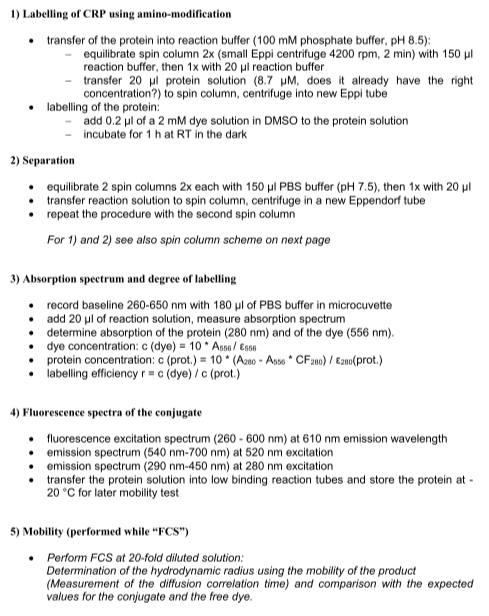
\includegraphics[width=0.6\textwidth]{protocol.png}
    \caption{Protocol for the Experiment }
    \label{fig:ViolinPlot}
\end{figure}

One notable difference is that the final Volume of collected protein at the end of Step 2, was 10µL instead of the expected 20 µL.

\chapter{Results and Discussion}
\label{cha:ResandDisc}

\section{Results}
\label{sec:material}
In the following section, we will discuss our results in the order suggested by the laboratory manual. 

We can see the Formulas used to calculate Dye Concentration (4.1) , Protien Concentration (4.2) and the resulting Labeling Efficiency (4.3).

We determined the Labeling efficiency to be 9.325471121 using the following formulas and tables above.
We used 19 as a correction for the dilution factor since only 10 µL of Product was added to 180 µL of Phosphate Buffer Solution (PBS) solution for the Spectral Measurement.

\begin{equation}
    C_{\text{dye}} = \text{DF} \cdot \left( \frac{A_{556}}{\epsilon_{556}} \right)
\end{equation}

where:\\
$C_{\text{dye}}$ = Dye Concentration ( Molar) \\
$\text{DF}$ = Dilution  Factor\\
$A_{556}$ = Absorption at 556 nm\\
$\epsilon_{556}$ = Emission at 556 nm\\


We determined the Dye concentration to be : 5.389 µM\\

We used 19 as a correction for the dilution factor since only 10 µL of final Product(Protein + Dye after Spin Column) was added to 180 µL of Phosphate Buffer Solution (PBS) solution for the Spectral Measurement.


\begin{equation}
    C_{\text{prot}} = \text{DF} \cdot \left( \frac{A_{280} - (A_{556} * \text{CF}_{280})}{\epsilon_{280}^{\text{prot}}} \right)
\end{equation}
where:\\
$ C_{\text{prot}}$ =  Protein Concentration (Molar)\\
$\text{DF}$ = Dilution  Factor\\
$A_{280}$ = Absorption at 280 nm\\
$A_{556}$ = Absorption at 556 nm\\
$ \text{CF}_{280})$ = Dye Correction Factor at 280 nm\\
$\epsilon_{280}$ = Computed Protein Emission at 280 nm\\


We determined the Protein Concentration to be :  0.5778 µM\\

We used 19 as the dilution factor since only 10 µL of final Product(Protein + Dye after Spin Column) was added to 180 µL of Phosphate Buffer Solution (PBS) solution for the Spectral Measurement.

\begin{equation}
R = \frac{C_{\text{dye}}}{C_{\text{prot}}}
\end{equation}
where:\\

$R$ = Labeling Efficiency ( Absolute Value )\\
$C_{\text{dye}}$ = Dye Concentration ( Molar )\\
$C_{\text{prot}}$ = Protein Concentration ( Molar )\\

We determined the Labeling efficiency  R to be:  9.325 \\
( Absolute Value of average Dye Molecules per Protein ) using the previous formula(4.3).





\begin{figure}[H]
    \centering
    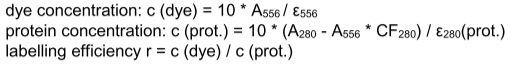
\includegraphics[width=0.6\textwidth]{labelingefficiency.png}
    \caption{Formulas Employed to Calculate Labeling Efficiency}
    \label{fig:ViolinPlot}
\end{figure}

We computed the Extinction Coefficient of our Protein using the Sequence and the following formula ( 4.2 ):

\begin{equation}
    \epsilon_{280}^{\text{Protein}} = n \cdot \epsilon_{280}^Y + m \cdot \epsilon_{280}^W
\end{equation}
\\
where:\\
$\epsilon_{280}^{\text{Protein}}$  =  Extinction Coefficient at 280 nm for BSA.\\
n = Coefficient for the molar absorptivity of tyrosine .\\
m = Coefficient for the molar absorptivity of tryptophan .\\
\\
The computed $\epsilon_{280}^{\text{Protein}}$ to be : $49180 M^-1cm^-1$ \\

We also used an online tool [4]  to calculate the Extinction Coefficient of our Protein ( BSA ) based on the sequence that we acquired from the UniProt Databank [3], which gave a slightly different result, which could be because of the addition of a minor absorption coefficient for Cysteine Residues as well.

\begin{figure}[H]
    \centering
    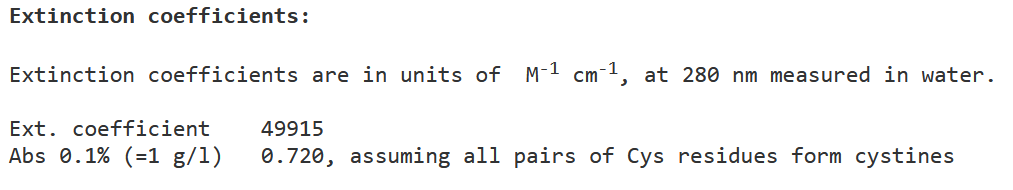
\includegraphics[width=0.6\textwidth]{extinctioncoefficient.png}
    \caption{Extinction Coefficient at 280nm calculated with Expasy ProtParam tool [4]}
    \label{fig:ViolinPlot}
\end{figure}

The probability of a protein has k dye labels follows follows Poisson distribution [5]:\\
\begin{equation}
    (P(k,\lambda) = \frac{\lambda^k e^{-\lambda}}{k!})\\
\end{equation}
\\
where $\lambda$ is the average of the labeled protein.
\\
The $\lambda$ here is the labeling efficiency(the ratio of dye molecules to protein molecule).\\



After that, the probability of non-labeled, single labeled and double-labeled proteins are derived as $P(k = 0), P(k = 1) and P( k = 2)$ giving a probability of 0.009\% of not being Labeled, a probability of 0.083\% of being Labeled with 1 dye molecule , and finally a probability of 0.388\% of being labeled with exactly 2 molecules.\\
\begin{table}[h]
    \centering
    \begin{tabular}{l|l}
        \toprule
        \textbf{Event} & \textbf{Probability (\%)} \\
        \midrule
        Not Labeled $P(k = 0)$ & 0.009\% \\
        Single Labeled $P(k = 1)$ & 0.083\% \\
        Double Labeled $P(k = 2)$ & 0.388\% \\
        \bottomrule
    \end{tabular}
    \caption{Probability Distribution for Protein Labeling}
    \label{tab:protein_labeling}
\end{table}

The final protein yield from the amount of used protein initially is 63.09\%
It was calculated by the Ratio of final protein Moles and initial protein Moles.
\\
We determined the emission spectrum (Fig. 4.3) of our product using the Spectrometer QEP02146.
\begin{figure}[H]
    \centering
    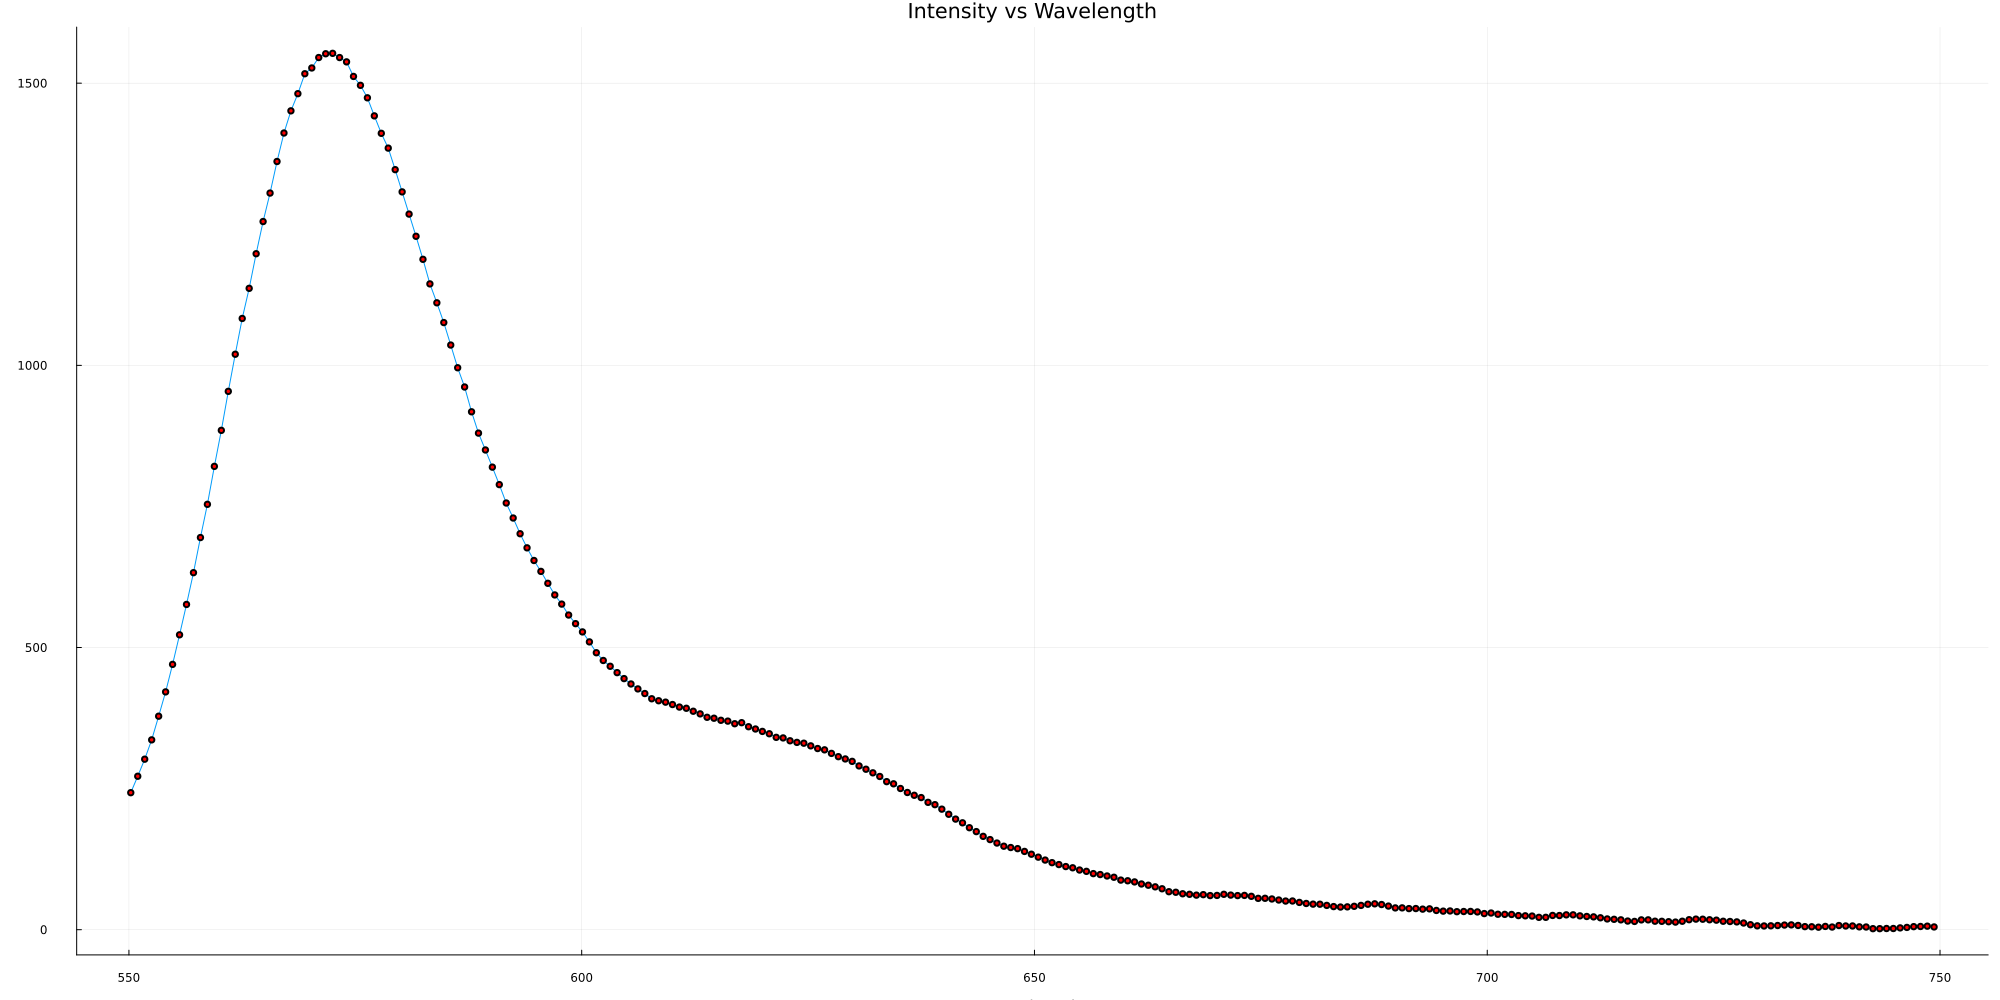
\includegraphics[width=0.95\textwidth]{emission.png}
    \caption{Emission Spectrum of Alexafluor546 labeled BSA: X-Axis is Wavelength and Y-Axis is Intensity}
    \label{fig:ViolinPlot}
\end{figure}

We determined the absorption spectrum (Fig. 4.4) of our product relative to a baseline containing only PBS using 

\begin{figure}[H]
    \centering
    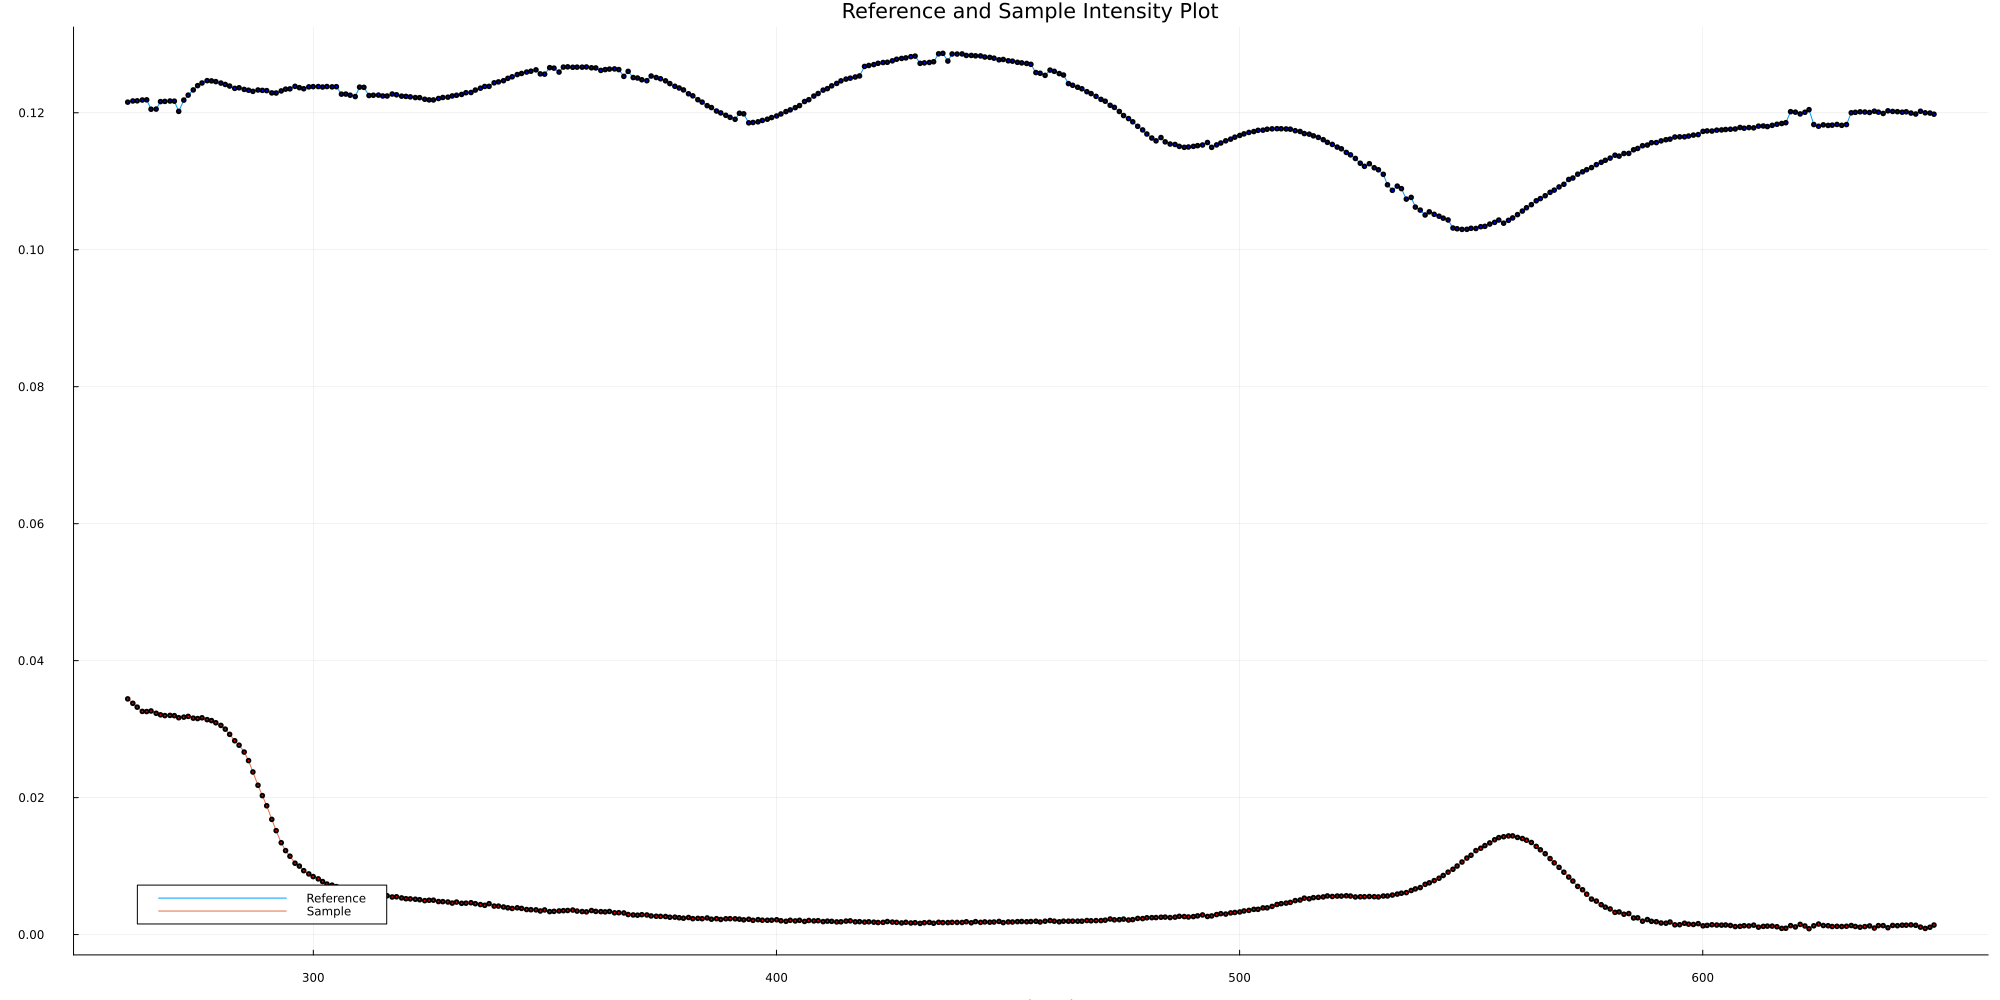
\includegraphics[width=0.95\textwidth]{Absorption of Reference and Sample.png}
    \caption{Absorption Spectrum of Alexafluor546 labeled BSA: X-Axis is Wavelength and Y-Axis is Intensity}
    \label{fig:ViolinPlot}
\end{figure}

We can use the known Hydrodynamic radius of Rhodamine 6G (0.59 nm) , it´s molecular weight of 470 Dalton and the known molecular weight of our protein, based on it´s sequence , of 69293.41 Daltons.  to calculate the Hydrondinamic Radius for our labeled protein (BSA).
To calculate the Hydronamic radii  we can use this formula:
\begin{figure}[H]
    \centering
    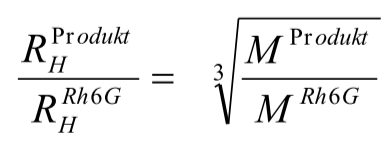
\includegraphics[width=0.3\textwidth]{hydronimacradius.png}
    \label{fig:ViolinPlot}
\end{figure}

The resulting hydrodynamic radius for Bovine Serum Albumin is: 5.28 nm 

We apply the same calculation on the  C-reactive protein(CRP). The molecular weight of monomer CRP is approximately 23kDa, which is one fifth of the pentamer. The resulting hydrodynamic radius for monomer CRP is 2.16nm, and the hydrodynamic radius for pentamer CRP is 3.69nm.

We can also use a hydrodynamic simulator [6] based on a structure of our protein to perform the same calculation, resulting in a Hydrodynamic radius of 4.68nm for the protein in an anhydrous condition.

\begin{figure}[H]
    \centering
    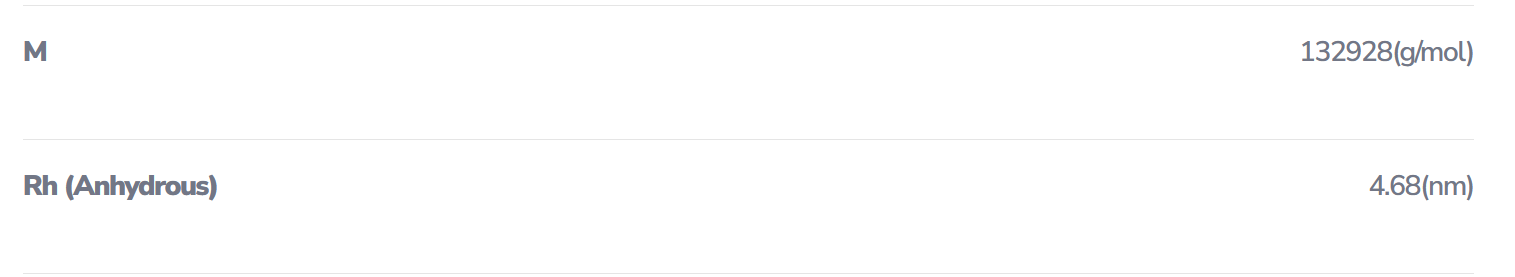
\includegraphics[width=0.8\textwidth]{Calculator.png}
    \label{fig:ViolinPlot}
\end{figure}


\section{Discussion}
\label{sec:methods}


 In the following part, we will discuss different aspects of our experimental results more in detail and answer specific questions contained in the experiment Script.
 The first argument we shall discuss is the relationship between absorption and emission spectra, that can be effectively explained by a Jablonski Diagram. 
 
 The Jablonski diagram [7] is a schematic representation of the energy levels of a molecule and the transitions between these levels. The energy levels in a Jablonski Diagram can be of various nature, the first and most important ones are the electronic energy levels (or rather the resulting molecular orbitals)followed by rotational energy levels and finally vibrational energy levels. The diagram is arranged vertically with increasing energy levels, and the transitions between the levels are represented by arrows. The absorption spectrum of a molecule is a plot of the amount of light absorbed by the molecule as a function of the wavelength of the light. The absorption spectrum is related to the Jablonski diagram because the absorption of light by the molecule causes the excitation of electrons from the ground state to higher energy levels. An upward arrow in the Jablonski diagram represents the excitation of the electrons. The emission spectrum of a molecule is a plot of the amount of light emitted by the molecule as a function of the wavelength of the light. The emission spectrum is related to the Jablonski diagram because the relaxation of the excited electrons to the ground state causes the emission of light at specific wavelengths. A downward arrow in the Jablonski diagram represents the relaxation of the electrons.
 
 \begin{figure}[H]
    \centering
    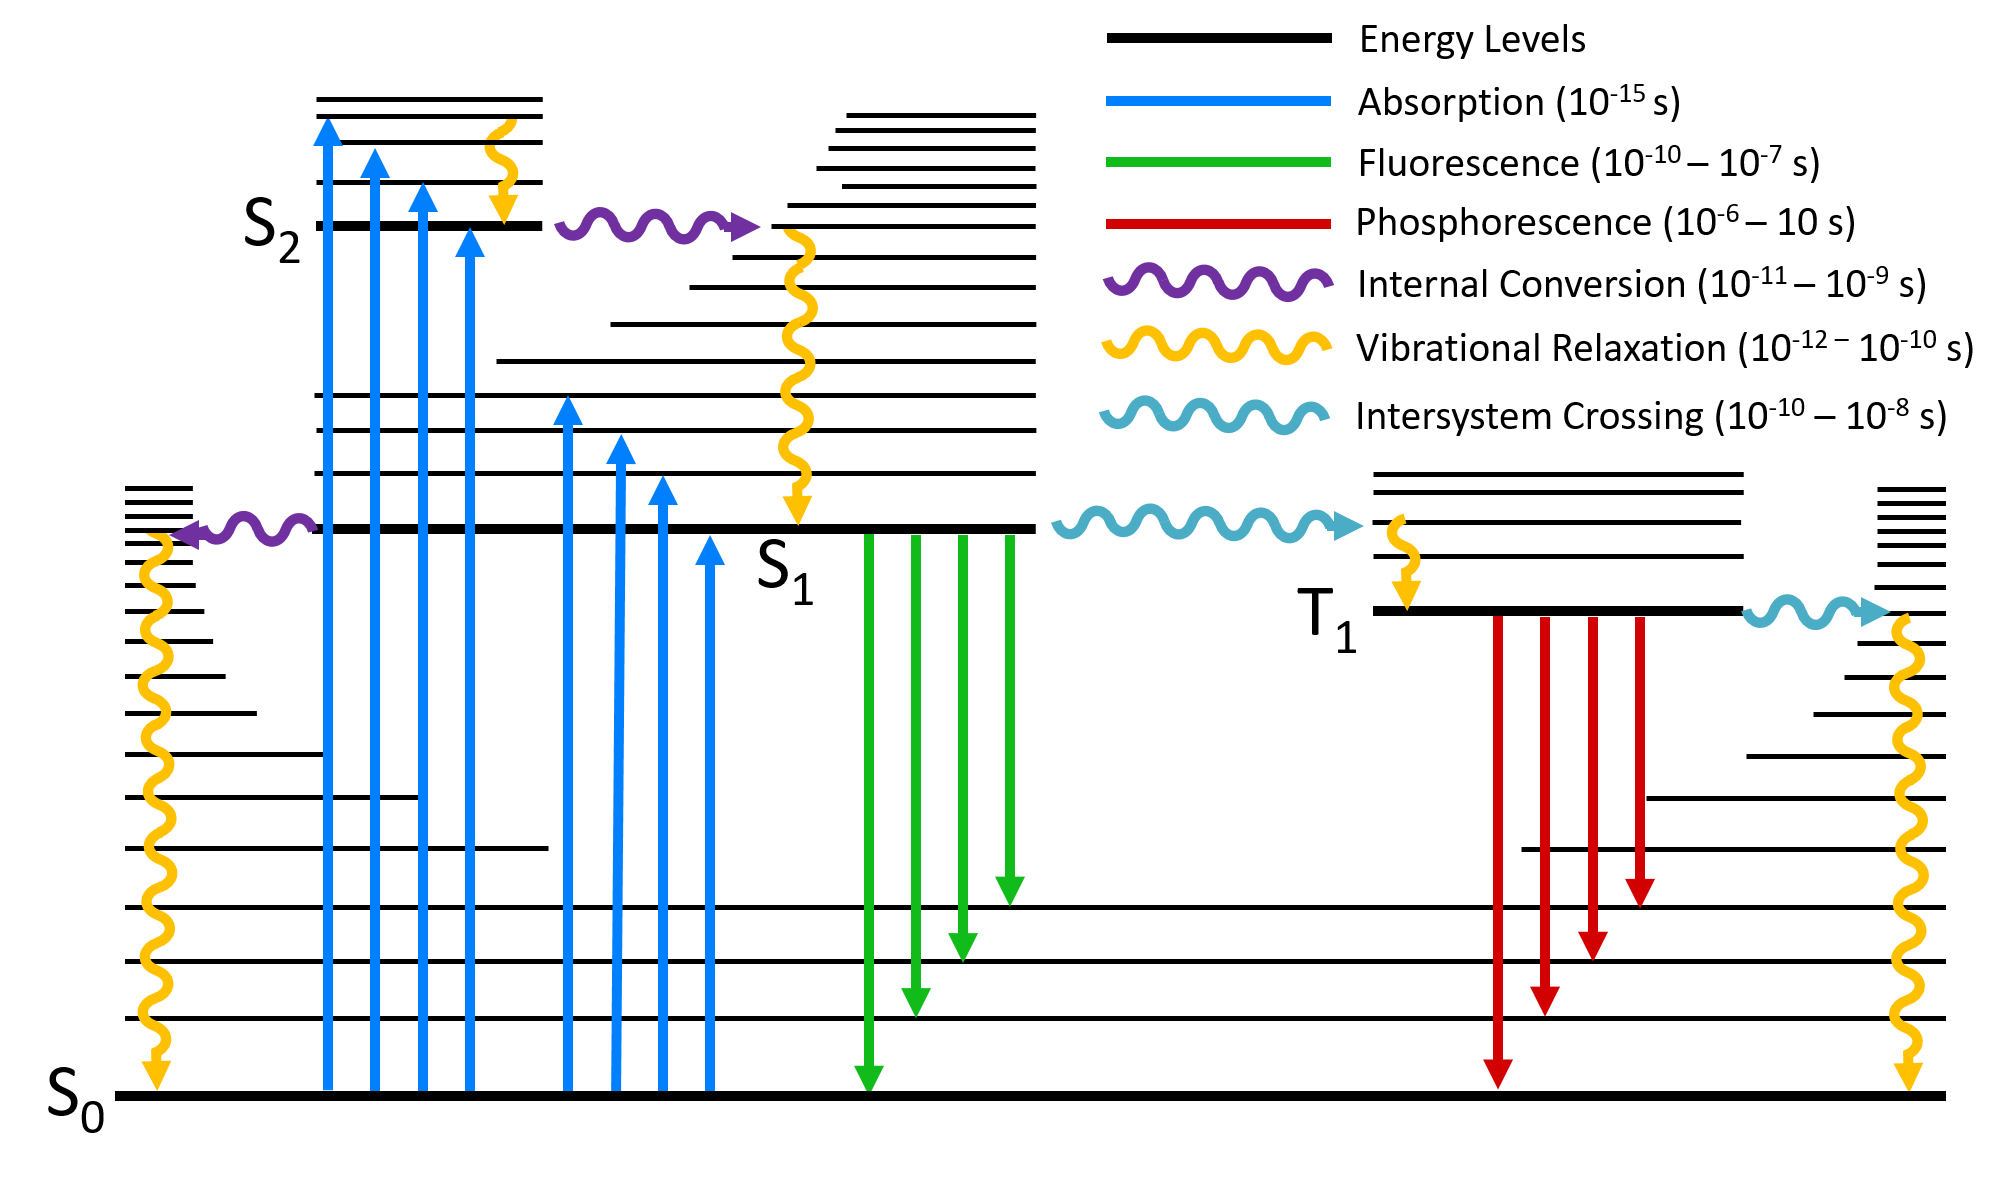
\includegraphics[width=0.8\textwidth]{Jablonski-Diagram-1-3523343705.png}
    \caption{Jablonski Diagram displaying Excitation, Fluorescent Emission, and Phosphorescent Emission} 
    \label{fig:ViolinPlot}
\end{figure}

The absorption and emission spectra of a labeled protein are related to each other because the wavelength of the absorbed light determines the energy of the excited state of the molecule, which in turn determines the wavelength of the emitted light . The relationship between the absorption and emission spectra is described by the Stokes shift, which is the difference between the excitation wavelength and the emission wavelength . The Stokes shift is caused by the relaxation of the excited state of the molecule to the ground state, which results in the emission of a photon with lower energy than the absorbed photon . The Stokes shift is an important parameter for characterizing fluorescent dyes because it affects the sensitivity and selectivity of fluorescence measurements.[15]It could also be due to a variety of factors such as the solvent used and the pH of the solution. 
\\
The shift could also be due to the labeling efficiency of the protein, which can affect the number of dye molecules attached to the protein and the position of the dye on the protein.


The observed labeling efficiency  could be influenced by various factors in the experimental process, variations in reaction conditions such as temperature, pH, or reaction time could impact the labeling efficiency, and we should consider the stability of the protein in it´s native state after being treated with a solution of pH of 8,5.
The correction factor of 19 used for the dilution factor indicates that a small volume of the labeled product was added to a larger volume of the PBS solution during spectral measurement. 
Other factors to consider include the quality and purity of reagents, as impurities can affect the labeling reaction. Additionally, the accuracy of measurements and pipetting during the experimental procedure may contribute to variations in the results.

To enhance accuracy, one could explore optimizing reaction conditions, ensuring thorough mixing during the labeling reaction, and verifying the purity of reagents. Replicating the experiment and averaging results could also improve reliability.

Moving forward, in the probability distribution calculation, the assumption of a Poisson distribution could be further validated. Comparing the theoretical distribution to experimental results may provide insights into the accuracy of this statistical model. Alternatively, exploring other statistical models that might better fit the experimental data could lead to a more accurate representation.
Additionally, exploring different methods for calculating protein yield, such as alternative quantitative techniques or incorporating quality control measures, might contribute to a more robust and reliable outcome.
The most significant challenge arose during the gel filtration process where we didn't obtain the expected 20µL. This discrepancy could be due to issues such as incomplete elution or sample loss during the process. 





\chapter{Conclusions}
\label{cha:conclusions}

In conclusion, fluorescence-based techniques have become indispensable in various scientific applications, offering sensitive and specific tools for probing biological systems. FISH, FLIM, and FRET provide valuable insights into genetic research and cellular processes, enabling precise molecular mapping and real-time observation of molecular interactions.

Photosensitivity, a key consideration in fluorescence experiments, underscores the need to protect fluorophores from excessive excitation cycles. This precaution is particularly pertinent for dyes like Alexa-Fluor, known for their limited excitation cycles before experiencing photobleaching.

Our experiment employed Alexa-Fluor 546, leveraging amino modification for stable protein labeling. Gel filtration chromatography, akin to molecular sieves, facilitated the separation of labeled proteins. Despite challenges, such as an unexpected volume discrepancy during gel filtration, we successfully calculated the labeling efficiency and explored various aspects of spectral analysis.

The observed labeling efficiency may be influenced by experimental conditions, reagent quality, and procedural nuances. Potential improvements involve optimizing reaction conditions, meticulous mixing during reactions, and verifying reagent purity. Moreover, addressing discrepancies in experimental outcomes, such as the gel filtration volume issue, requires careful procedure monitoring and optimization.

Looking ahead, our experiment's next phase involves Fluorescence Correlation Spectroscopy (FCS) to validate conjugation.


\chapter{References}
\label{cha:References}

[1] Gel-Filtration Chromatography | SpringerLink. https://link.springer.com/protocol/10.1007/978-1-4939-6412-32.
\newline[2] The Beer-Lambert Law - Chemistry LibreTexts. https://chem.libretexts.org/Bookshelves/TheBeerLambertLaw.
\newline[3] BSA Uniprot Entry and sequence: https://www.uniprot.org/uniprotkb/P02769/entryfunction
\newline[4]Tool used to calculate extinction coefficient https://web.expasy.org/cgi-bin/protparam/protparam
\newline[5] Poisson Dsitribution: https://en.wikipedia.org/wiki/Poissondistribution
\newline[6] Hydronamic Radius Calculator :https://www.fluidic.com/resource/hydrodynamicradiuscalculations/
\newline[7] Jablonski Diagram entry : https://en.wikipedia.org/wiki/Jablonskidiagram
\newline[8] Stokes Shift : https://en.wikipedia.org/wiki/Stokesshift
\newline[9] https://en.wikipedia.org/wiki/Fluorescenceinsituhybridization
\newline[10] https://en.wikipedia.org/wiki/Fluorescence-lifetimeimagingmicroscopy
\newline[11] https://en.wikipedia.org/wiki/F\%C3\%B6rsterresonanceenergytransfer
\newline[12] https://www.thermofisher.com/order/catalog/product/A20002
\newline[13] https://www.uniprot.org/uniprotkb/P02769/entry
\newline[14] A Comprehensive Review of Fluorescence Correlation Spectroscopy -Front. Phys., 12 April 2021 Sec. Optics and Photonics Volume 9 - 2021 | https://doi.org/10.3389/fphy.2021.644450
\newline[15] A fluorescent dye with large Stokes shift and high stability: synthesis and application to live cell imaging DOI: 10.1039/C6RA27547H (Paper) RSC Adv., 2017, 7, 7604-7609
\end{document}
